% Para documento texto corto
\documentclass[paper=a4,oneside,fontsize=12pt]{article}
%\documentclass[paper=letter,oneside,fontsize=12pt, 
% parskip=full]{scrartcl}

% Establecer dimensiones de los margenes
%\ usepackage[inner=1.5cm,outer=3cm,top=2cm,bottom=4cm,
%	bindingoffset=5mm]{geometry}
\usepackage[left=3cm,right=3cm,top=3cm,bottom=3cm,
bindingoffset=0cm]{geometry}

% Permite ingresar caracteres acentuados y especiales 
% sin necesidad de emplear comando
% utf8 codificacion de entrada Unicode (mas simbolos que ASCII)
\usepackage[utf8]{inputenc}

% T1 encoding for European, English, American text
\usepackage[T1]{fontenc}
% Fuente escalable
\usepackage{lmodern}

% Carga babel, idioma ingles
\usepackage[english,spanish]{babel}

% Mejor jsutificacion, tipografia alta calidad.
\usepackage{microtype}
% Para unir columnas y filas en tablas
\usepackage{array}

% Agrega comandos extra al comando tabular
% \toprule, \midrule, \bottomrule
\usepackage{booktabs}
% Tablas con ancho establecido por usuario
\usepackage{tabularx}
% Para posicionamiento preciso de tablas dentro del texto
\usepackage{float}

% Encabezados personalizados
\usepackage{fancyhdr}
\usepackage{graphicx}

% Permite obtener el numero de la ultima pagina
\usepackage{lastpage}

% Paquetes para figuras
% Paquete caption para titulos figuras
% Paquete subcaption para subfiguras
\usepackage{caption}
\usepackage{subcaption}

% Espaciado inteligente
\usepackage{xspace} 

% Cabeceras
\pagestyle{fancy}
% Borra cabecera y pie actuales
\fancyhead{}
% Cintillo cabecera
%\chead{
%	
\includegraphics[width=150mm]{Imagenes/Cabecera.png}
%}
\fancyhead[L]{
\includegraphics[width=\textwidth]{Imagenes/Cabecera.png}}
\fancyfoot[C]{ 
	\begin{tabularx}{\textwidth}{|X|m{10cm}|m{1.2cm}|}
		\hline
		\centering Versión 0.1	& 
		\centering 
\includegraphics[height=0.8cm]{Imagenes/Pie.png} & 	
		\thepage~/~\pageref{LastPage} \\			
		\hline 
	\end{tabularx}	
}

% Numeracion de paginas
% numeros arabigos
\pagenumbering{arabic}

% Comando que define el nombre la aplicacion
\newcommand{\AppName}{\textsc{CenditLab}\xspace}

% Comando que define el nombre del sistema de medición de figura de ruido
\newcommand{\smr}{sistema de medición de ruido}
\newcommand{\SMR}{SMR\xspace}

% Comando que define el nombre del Cendit
\newcommand{\cendit}{Cendit\xspace}

\begin{document}
	
	%\begin{titlepage}		
		%Pagina de titulo		
		\begin{center} 			
			% Titulo parte superior
			\begin{Large} 
				\textsc{Dirección de Servicios de Certificación}
				\\[5pt]
				\textsc{Laboratorio de Ensayos de Compatibilidad Electromagnética Radiada}
			\end{Large}
				
				\vspace{10cm}
			% Titulo central
			\begin{LARGE}			
				\textsc{Especificación de Requerimientos de Software}
			\end{LARGE}
		
			\vspace{8pt}
		
			\begin{Huge}
				\textsc{\AppName}
			\end{Huge}
		
			% Tabla para revisores
			\begin{table}[!b]
				\begin{tabularx}{\linewidth}{|X|X|X|X|}	
					\hline				
					\multicolumn{2}{|l|}{\textbf{FORMATO}: } & \multicolumn{2}{|l|}{\textbf{N DOC:}} \\
					\hline
					Originado por:	& Elaborado por: & Revisado por: & Aprobado por: \\
					\hline
					Br. Arias B., Jose A. & Br. Arias B., Jose A. & - & - \\
					\hline
					\textbf{Fecha: 16/06/2017} & \textbf{Fecha: 16/06/2017} & & \\				
					\hline
				\end{tabularx}	
			\end{table}		
		
		\end{center}
		
	%\end{titlepage}
	
	% Salto de pagina
	\clearpage
	
	% Indice 
	\tableofcontents
	
	% Salto de pagina
	\clearpage
	
	% Espaciado entre parrafos
	\setlength{\parskip}{0.5em}
	
	\section{Introducción}
	Esta sección brinda un panorama general del contenido del presente documento de especificaciones de requisitos de software. Se da al final una lista de abreviaturas.
	
	\subsection{Propósito}
	El propósito de este documento es dar una descripción detallada de los requerimientos para el software \AppName. Ilustrará el propósito y sentará de manera formal y completa los requerimientos que debe poseer el software \AppName establecido por los usuarios de \smr en el \cendit. Este documento servirá como base inicial para el proceso de desarrollo. Explicará la restricciones del sistema, interfaces e interacciones con aplicaciones externas. 
	
	Este documento se dirige principalmente a los futuros usuarios de la software \AppName para fines de aprobación, y para desarrolladores, que se involucren en un futuro en el soporte y mejoras de la base de código.
	
	\subsection{Alcance}
	
	El software \AppName es una aplicación para PC de escritorio que servirá que reunirá la funcionalidad que brindan los tres equipos principales que conforman el \smr en una interfaz de software única y centralizada.  
	
	\AppName permitirá realizar las tareas propias de medición que comúnmente un usuario ejecuta frente al \SMR físico pero ahora desde una aplicación de software: un entorno de software o laboratorio virtual que permitirá replicar la funcionalidad de los instrumentos del \SMR y aumentar sus capacidades.	

	El proceso de medición puede necesitar de la ejecución múltiples etapas que, desde el punto de vista de la aplicación, pueden resumirse en dos: calibración de los instrumentos y realización de la medición. Así que el principal objetivo de \AppName será el de asistir al usuario en la configuración de la instrumentación y automatizar el proceso de inicio a fin, en todas sus etapas.		
	
	El principal objetivo para el diseño de la aplicación \AppName es el de automatizar el proceso de medición con los instrumentos del \SMR de inicio a fin. 
	
	Por medio de \AppName el usuario podrá inspeccionar que instrumentos se encuentran conectados a los buses de datos, conocer cuales de ellos se encuentran activos o inactivos, establecer su configuración, realizar mediciones, captura y visualización datos, programar tareas de medición empleado comandos SCPI además de generar reportes con resultados en formatos digitales, como pdf o html. 
	
	% BEGIN review	
	\AppName permite a los usuarios realizar mediciones de manera automatizada y remota, configuración los instrumentos instrumentos del \smr, capturar y visualizar de datos además de generar reportes en formatos digitales, como pdf o html.
	% END review
	
	\AppName utiliza la capacidad de transferencia de datos a través de buses de comunicaciones que disponen los instrumentos del \smr, como GPIB, USB o LAN. Para ello el PC donde se ejecute la aplicación debe disponer de los aditamentos de hardware apropiados que permitan acceder a estos buses, así como también el respectivo soporte de software en forma de librerías o controladores de dispositivo, que permitan a un PC el acceso a estos buses.
	
	\subsection{Definiciones, acrónimos y abreviaturas}
	
	\begin{table}[h!]
		\begin{tabularx}{\textwidth}{|c|X|} 
			\hline
			\textbf{Término} & \textbf{Definición} \\
			\hline
			Stakeholder & Participante \\
			\hline
			VM	& Virtual Machine, maquina virtual que se encarga de ejecutar una aplicación \\
			\hline
			JVM & Java Virtual Machine \\
			\hline
			UML & Unified Modeling Language, lenguaje unificado de modelado, permite modelar gráficamente la estructura y comportamiento de unidades de software \\
			\hline
			SO & Sistema Operativo \\
			\hline
		\end{tabularx}	
	\end{table}

	\subsection{Referencias}
	% 	\bibliographystyle{acm}	
	% 	\bibliographystyle{abbrv}	
	% 	\bibliographystyle{apalike}
	
	%\bibliographystyle{ieeetr}
	%\bibliography{Bibliografia}
	
	\begingroup
		\renewcommand{\section}[2]{}
		\begin{thebibliography}{9}
			\bibitem{iso-29148} 
			ISO/IEC/IEEE 29148. 
			\textit{Systems and Software Engineering - Lyfe Cycle Processes - Requirements Enginering}. 
			ISO/IEC/IEEE, 2011.
			
			\bibitem{iso-42010} 
			ISO/IEC/IEEE 42010. 
			\textit{Systems and Software Engineering - Architecture Description}. 
			ISO/IEC/IEEE, 2011.		
			
			\bibitem{softwareengineering-narang} 
			Rajesh Narang. 
			\textit{Software Engineering Principles and Practices}. 
			Mc Graw Hill, New Delhi, India, 2015.			
			
			\bibitem{softwareengineering-sommerville} 
			Ian Sommerville. 
			\textit{Software Engineering}. 
			Addison-Wesley, Boston, Massachusetts, 2011.				

		\end{thebibliography}
	\endgroup
	
	\subsection{Visión general}
	
	El resto de este documento incluye tres capítulos y un apéndice. El segundo provee un panorama de la funcionalidad de la aplicación de software y su interacción con el \smr. Este capitulo además introduce los diferentes tipos de \emph{participantes} y su interacción con el sistema. Más adelante, el capitulo menciona las restricciones del sistema y las suposiciones de la aplicación.
	
	El tercer capitulo describe la especificación de requerimientos al detalle y describe las diferentes interfaces del sistema. Se emplean diferentes técnicas de especificación con el objeto de mostrar los requerimientos de manera precisa para distintas audiencias.
	
	El cuarto capitulo trata con el establecimiento de la prioridad de los requerimientos. Este incluye una motivación. Expone los motivos para los métodos de prioridad escogidos y el por que de las alternativas rechazadas.  
	
	El apéndice al final de este documento incluye los resultados de la priorización de requerimientos y el plan de entrega basado en las prioridades.
	
	\section{Descripción general}
	
	Esta sección brindará una perspectiva general de todo el sistema de software \AppName. El sistema será explicado dentro de su contexto para mostrar como éste interactúa con el \smr por medio de su funcionalidad básica. Describirá además que tipo de participantes \textendash \emph{stakeholders} \textendash usarán el sistema y que funcionalidad estará disponible para cada tipo de ellos. Al final, se presentan las restricciones y suposiciones para el sistema.
	
	\subsection{Perspectiva de producto}
	
	\AppName será un aplicación de escritorio que brindará una interfaz de software de la funcionalidad que proporcionan los instrumentos físicos presentes en el \smr.
	
	% Revisar
	\AppName será un aplicación de escritorio que servirá como interfaz de usuario de software para el \smr.
	% Revisar
	
	En la figura \ref{Fig:SystemMainDiagram} se muestra como la aplicación de software \AppName de la izquierda se integra a los instrumentos de hardware que conforman el \smr en la derecha, dando como resultado un sistema de mayores prestaciones. 
	
	La aplicación \AppName consta de cinco módulos de software principales. El módulo \emph{IO} se encarga de la gestión de la comunicación bidireccional de datos entre la aplicación y los instrumentos de medición. El módulo \emph{GUI} se encarga de la interfaz de usuario. \emph{EJECUCIÓN} es el módulo destinado a realizar las tareas de medición. El soporte en software para los instrumentos del \SMR lo brinda el módulo \emph{INSTRUMENTOS}. El módulo \emph{REPORTES} tiene la misión de generar documentos digitales que contengan los resultados del proceso de medición.		


	% Revisar
		Conceptualmente se ha dividido la aplicación en cuatro grandes paquetes, como ilustra el diagrama UML de la figura \ref{Fig:SystemMainDiagram}
	% Revisar
	
	\begin{figure}[H]
		\centering
		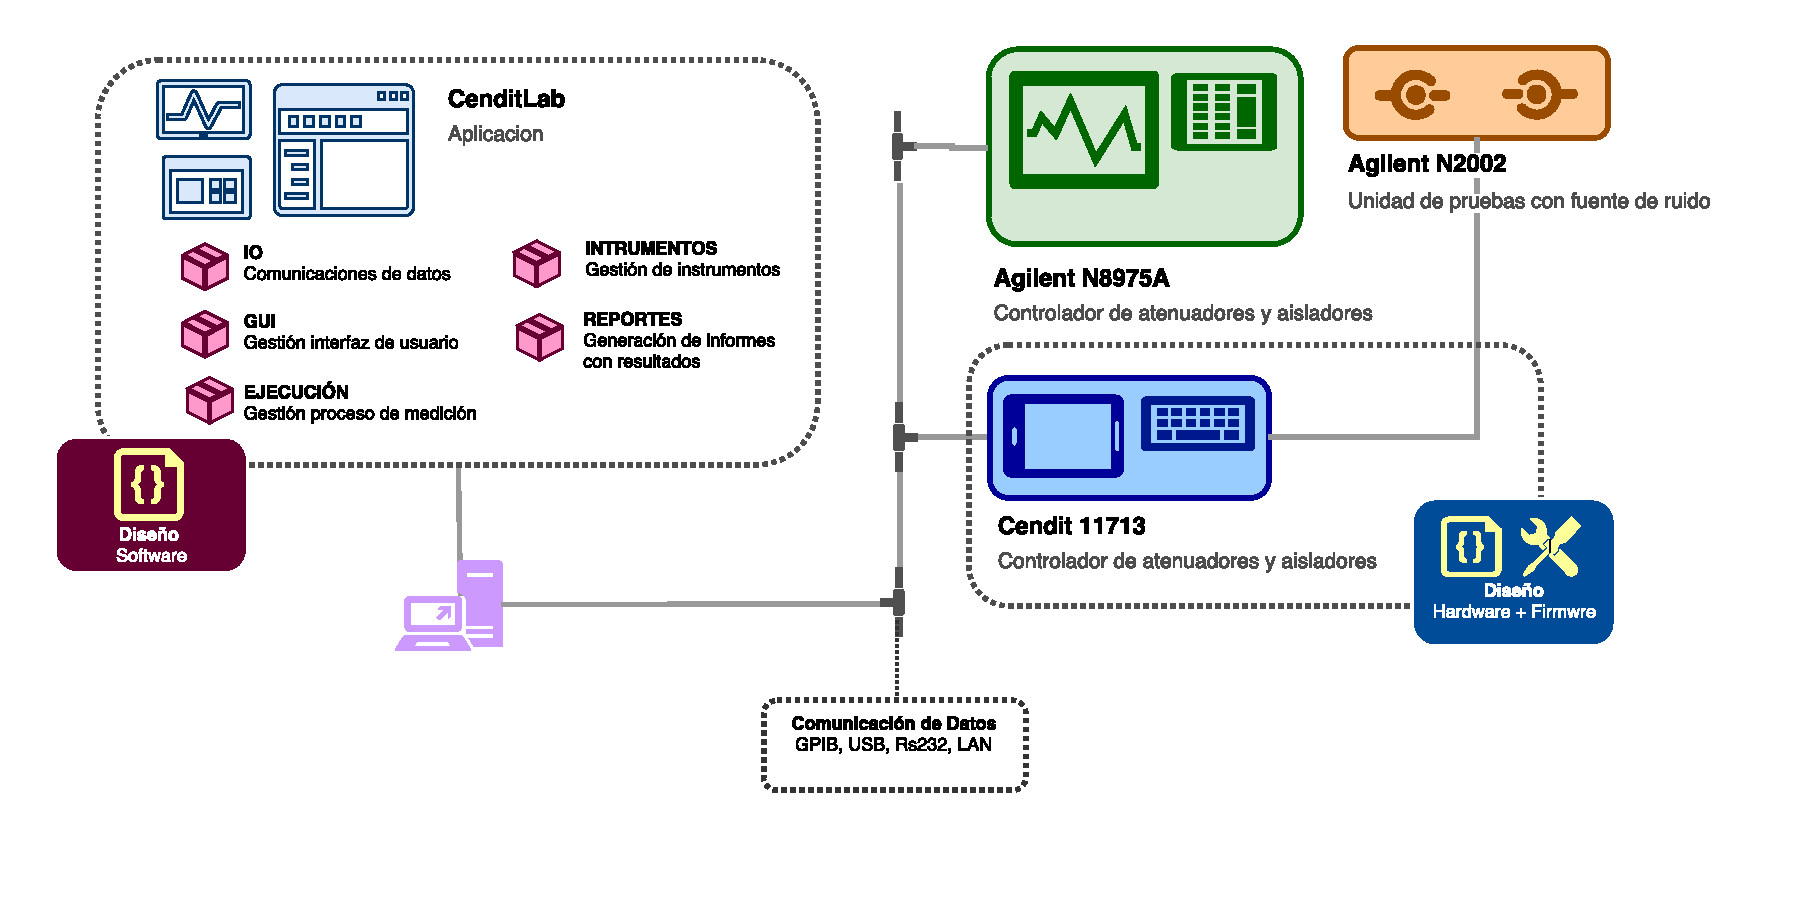
\includegraphics[width=15cm]{Imagenes/SystemMainDiagram.pdf}
		\caption{Diagrama bloques del sistema}
		\label{Fig:SystemMainDiagram}
	\end{figure}

	\begin{figure}[H]
		\centering 
		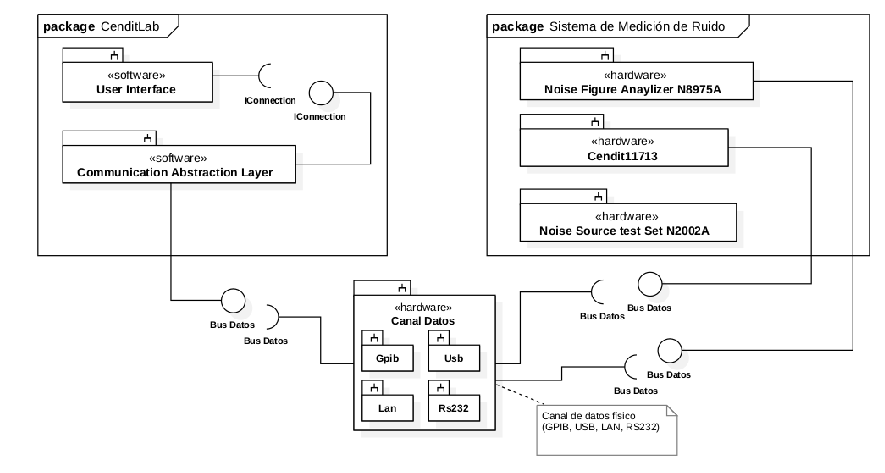
\includegraphics[width=15cm]{Imagenes/MainSystemPackagesUML.pdf}
		\caption{Diagrama UML del sistema}
		\label{Fig:MainSystemPackagesUML}
 	\end{figure}
 
 	La interfaz de usuario mostrará una representación visual de la configuración de instrumentos presentes en el \SMR para cada tarea de medición disponible en el software. Estará orientada a un formato de diagrama de bloques, donde cada instrumento estar representado por un bloque. El usuario podrá interactuar con cada uno de ellos para configurar el instrumento respectivo. La GUI servirá como guía de los pasos a seguir durante toda la secuencia de pasos a ejecutar durante la medición. En la figura \ref{Fig:SystemMainDiagram} el módulo \emph{GUI} dentro de la aplicación contiene el soporte de software para la interfaz de usuario.
 	
	La funcionalidad de los instrumentos que componen el \SMR sera representada en software por unidades funcionales que se llamarán  \emph{bloques de tareas}. El usuario, por medio de la interfaz gráfica, podrá configurar la instrumentación agregando, conectando y programando bloques de tareas. Es responsabilidad del paquete \emph{Procesamiento de Bloques de Tareas} la compilación y ejecución de la programación hecha por el usuario. 	

	En la \ref{Fig:SystemMainDiagram} el vinculo entre la aplicación de software y el hardware lo constituye el canal de \emph{Comunicación de Datos}. Es un enlace bidireccional que le permite a la aplicación intercambiar datos y comandos con los instrumentos. Este canal puede tomar la forma de bus de datos GPIB, USB, RS232 o una red LAN. El módulo \emph{IO} es la encargado de gestionar todo lo relativo a la comunicación de datos a través de múltiples interfaces o buses disponibles, mientras brinda una interfaz uniforme a las capas de software superiores.
	
	La aplicación \AppName presentará los resultados de una tarea de medición en pantalla o en documentos digitales, en formato de documento portable (pdf), en lenguaje de marcado de hipertexto (html) o en formato de texto plano, como valores separados por comas (csv). El módulo \emph{REPORTES} se encargará de cubrir esta funcionalidad.
	
	\AppName será una aplicación dirigida inicialmente a PC de escritorio que ejecute en una distribución de software libre, Linux principalmente, o un sistema operativo propietario, como Windows de Microsoft. Esto garantiza que \AppName será una aplicación portable, podrá ser ejecutada por cualquier equipo o dispositivo que posea una \emph{maquina virtual} apropiada, como JVM en Java o el entorno .NET de Microsoft, tecnologías que se encuentran disponibles bajo licencias de software libre.
	
	La aplicación resultará en una interfaz de software para los tres equipos principales que componen el \smr. En si resultará en un \emph{instrumento virtual} que concentra toda la funcionalidad del \SMR en un solo sitio: el dispositivo o PC que ejecute la aplicación.
	
	\subsection{Funciones de producto}
	
	Las tareas de medición que realizaría un usuario por medio de las interfaces físicas empleando de los instrumentos que conforman \SMR podrán realizarse a través \AppName, la cual brindará una única interfaz de software al \SMR. 
	
	A través de \AppName no se necesita presencia física del usuario en el \SMR, la aplicación brindará acceso remoto a través de buses de comunicación de datos o por red LAN. 
	
	La aplicación se encargará de buscar y presentar al usuario los instrumentos que forman \SMR que se encuentren en linea, es decir, conectados a un bus de datos o a una red LAN, a la cual la PC donde se ejecute la aplicación tenga la facilidad de acceso.
	
	La funcionalidad principal de \AppName será la de automatizar el proceso de medición con el \SMR. 
	
	La interfaz gráfica de la aplicación permitirá al usuario seleccionar los instrumentos en linea y así configurar la instrumentación adecuada para la tarea de medición, por medio de la representación gráfica de los instrumentos en forma de diagrama de bloques. Estos bloques admiten programación en forma de comandos SCPI,  estándar para instrumentos programables.
	
	El usuario podrá ejecutar la secuencia de comandos y observar los resultados en tiempo real en pantalla. La aplicación podrá además guardar los resultados de la mediciones en formatos de documento digital como pdf, html o texto plano.		
	
	\subsection{Características de los usuarios}
	
	La aplicación \AppName está dirigida a usuarios con formación técnica en el tarea de radio frecuencia, comunicaciones, antenas, electrónica y afines. En estos campos se  consideran ingenieros y técnicos universitarios como \emph{usuarios técnicos} en este documento.
	
	\subsection{Restricciones}	
	
	La aplicación \AppName requiere que en el PC o dispositivo donde se ejecute se encuentre instalada la \emph{maquina virtual} adecuada y con la versión correcta (Java Virtual Machine, JVM para Java o el entorno .NET ). 
	
	\AppName hace uso intensivo de las comunicaciones a través de los buses GPIB, USB o través de una red LAN. Por ello en el dispositivo o PC donde se ejecuta la aplicación se requiere de los periféricos de hardware apropiados, como adaptadores USB a GPIB o puente LAN a GPIB. En software también se necesita el soporte apropiado para las comunicaciones de datos, requiere de las librerías VISA de National Instruments, Linux-GPIB, VXI-11 y libUSB.	

	\subsection{Suposiciones y dependencias}	
	
	Se parte del supuesto de que el dispositivo donde se ejecute la aplicación posee la cantidad de memoria adecuada y la capacidad de procesamiento necesario para que la maquina virtual ejecute la aplicación, sin una degradación del desempeño apreciable.
	
	\section{Requerimientos específicos}
	
	Esta sección presenta todos los requerimientos funcionales y de calidad para la aplicación \AppName. Muestra un descripción detallada del sistema y de todas sus características.
	
	\subsection{Requerimientos de interfaces externas}
	
	\subsubsection{Interfaces de usuario}
	
	Cuando el usuario inicia la aplicación, se mostrará la pantalla inicial de la figura \ref{Fig:MainWndowUI}. Esta ventana principal de la aplicación, representa el centro de control de la aplicación ya que concentra múltiples funciones en forma de controles de ventana, comúnmente llamados \emph{widgets}, que el usuario debe seleccionar para ejecutar la acción asociada este control. 
	
	\begin{figure}[]
		\centering 
		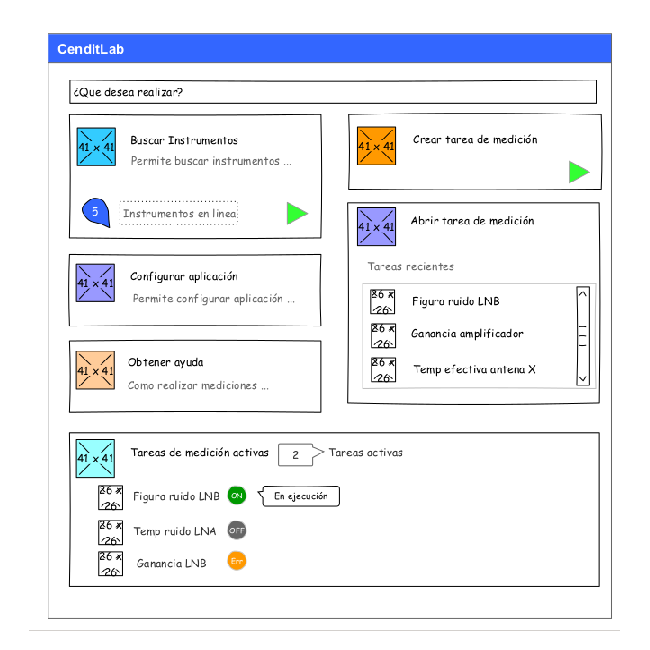
\includegraphics[width=10cm]{Imagenes/MainWindowUI.pdf}
		\label{Fig:MainWndowUI} 
		\caption{Sketch para la ventana principal de la aplicación}
	\end{figure}		
	
	En la pantalla un control en la ventana principal de la aplicación, sera llevado a otra ventana con la funcionalidad asociada al control. Por ejemplo, al seleccionar el control \emph{Buscar Instrumentos} se le presentará la ventana de \emph{Explorador de Instrumentos}. 
	
	\begin{figure}[H]
		\centering 
		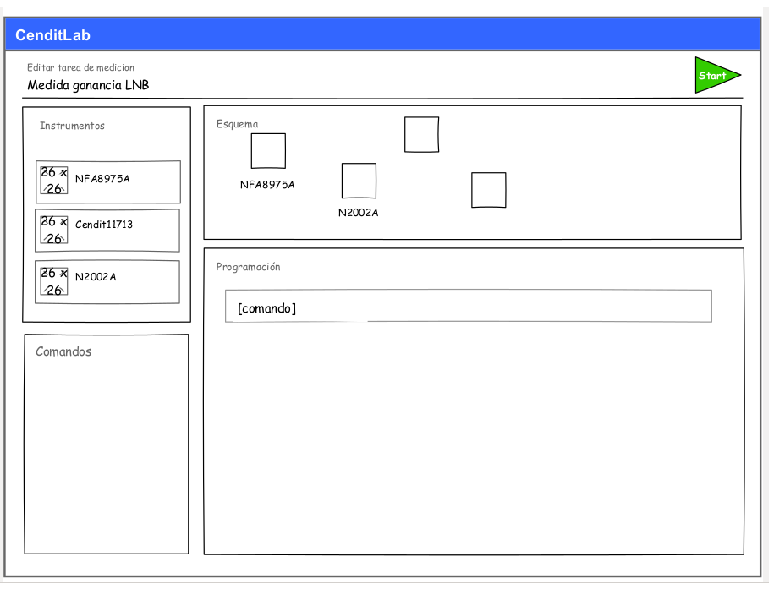
\includegraphics[width=10cm]{Imagenes/ProgramWindowUI.pdf}
		\caption{Sketch para la ventana de programación de tareas}
		\label{Fig:ProgramWindowUI} 		
	\end{figure}
	
	Al seleccionar \emph{Crear tarea} el usuario sera llevado a la ventana de programación de tareas de la figura \ref{Fig:ProgramWindowUI}. Por medio del control \emph{Abrir tarea} el usuario puede cargar una tarea de medición, previamente almacenada, a la ventana de programación. Presionando el control \emph{Configurar aplicación} se presentará la ventana en donde el usuario puede ajustar la configuración global de la aplicación. Presionando el control \emph{Obtener ayuda} se presentará una ventana en donde el usuario podrá indagar por ayuda.

	\begin{figure}[H]
		\centering 
		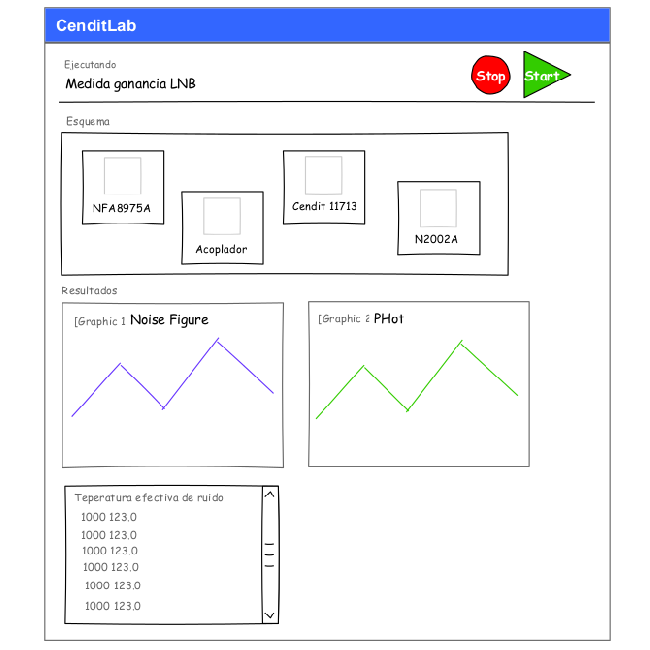
\includegraphics[width=12cm]{Imagenes/ExecutionWindowUI.pdf}
		\caption{Sketch para la ventana de ejecución de tareas}
		\label{Fig:ExecutionWindowUI} 		
	\end{figure}

	Dentro de la ventana de programación de tareas de la figura \ref{Fig:ProgramWindowUI} el usuario puede seleccionar los bloques que representan a los instrumentos y arrastrar cada bloque al panel de esquema (parte superior derecha), en donde puede configurar un diagrama de bloques con la instrumentación a utilizar para el proceso de medición. El panel de programación,  ubicado en la parte inferior derecha, permite realizar la programación de los instrumentos. El usuario selecciona bloques de instrucciones del panel inferior izquierdo a panel de programación. El usuario edita los comandos IEEE488 o SCPI dentro de los bloques de instrucciones. 

	Al presionar el botón \emph{start} en la ventana de la figura \ref{Fig:ProgramWindowUI} se procederá a ejecutar el programa y se mostrará la ventana de la figura \ref{Fig:ExecutionWindowUI}. En  esta ventana se muestran los resultados de las mediciones en timepo real.
	
	\subsubsection{Interfaces de hardware}
	
	La aplicación \AppName requiere un intercambio de datos continuo y confiables con el \smr. En la figura \ref{Fig:MainSystemPackagesUML} se muestra un diagrama compuesto UML que indica muestra los \emph{paquetes} de software (\AppName) y de hardware (\smr) y el \emph{canal de datos}, puente de comunicación entre estos dos paquetes.
	
	Se tiene una interfaz de hardware, el bus de datos, representada en la figura \ref{Fig:MainSystemPackagesUML} por los circulos y semicirculos con la etiqueta \texttt{Bus Datos}. Esta puede tomar la forma de buses Usb, Gpib, Rs232 o de una red Lan. Las interfaces de hardware la constituyen todos los dispositivos físico que deben estar presentes en el canal de datos, entre el computador que ejecuta la aplicación y los instrumentos que integran el \SMR.	
	
	\begin{figure}[H]
		\centering
		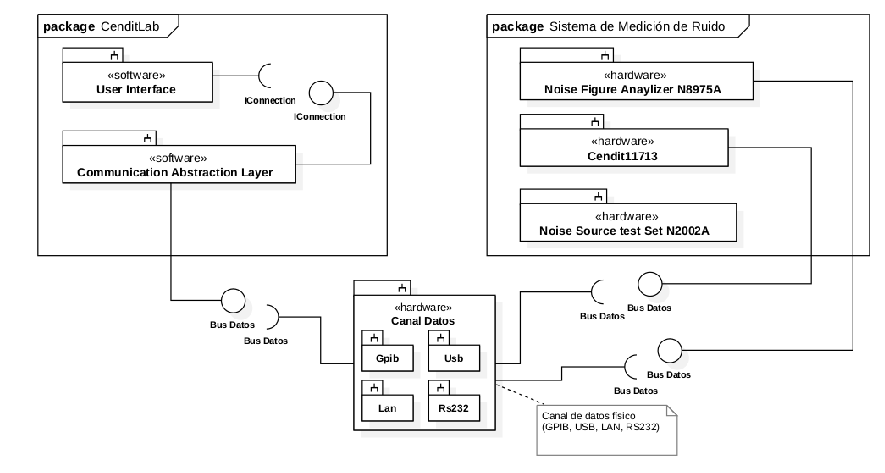
\includegraphics[width=0.8\textwidth]{Imagenes/MainSystemPackagesUML.pdf}
		\caption{Vista general de interfaces de software y hardware}
		\label{Fig:MainSystemPackagesUML2}
	\end{figure}
	
	\subsubsection{Interfaces de software}
	
	Dentro del \emph{marco de paquetes} etiquetado como \AppName de la figura \ref{Fig:MainSystemPackagesUML} se encuentra la principal interfaz de software, llamada \texttt{IConnection}. Esta interfaz representa una abstracción de alto nivel del canal de comunicaciones físicos, bien sea un bus Gpib, Usb, Rs232 o una conexión a red Lan. La interfaz \texttt{IConnection} es provista por una capa de sofware que se ha llamado como \texttt{Communication~Abstraction~Layer} y se indica en la figura \ref{Fig:MainSystemPackagesUML}, interfaz que será utilizada o consumida por niveles superiores dentro del software de \AppName.
	
	\begin{figure}[H]
		\centering
		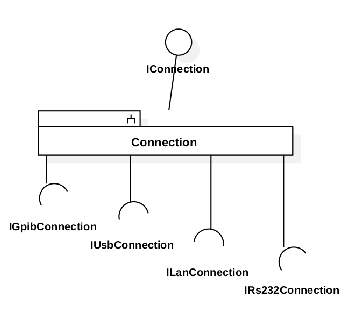
\includegraphics[width=0.4\textwidth]{Imagenes/CommunicationAbstractionLayerPackages1.pdf}
		\caption{Principales interfaces de software}
		\label{Fig:CalPackagesMain}
	\end{figure}
	
	El paquete de software \texttt{Communication~Abstraction~Layer}, como se muestra en la figura \ref{Fig:CalPackagesMain}, necesita consumir las interfaces \texttt{IGpibConnection}, \texttt{IUsbConnection}, \texttt{ILanConnection}, \texttt{IRs232Connection} que presentan funcionalidad de software para acceso a los respectivos buses de datos. 
	
	Cada una de las interfaces mencionadas requieren el uso de librerías nativas, instaladas en el sistema operativo donde se ejecute la aplicación. Estas representan interfaces de software que permiten el intercambio de datos a bajo nivel. La dependencia entre las librerías de alto nivel con sus respectivas librerias nativas se indica en las figuras \ref{Fig:CalPackages1} y \ref{Fig:CalPackages2}.

	\begin{figure}[H]
		\centering
		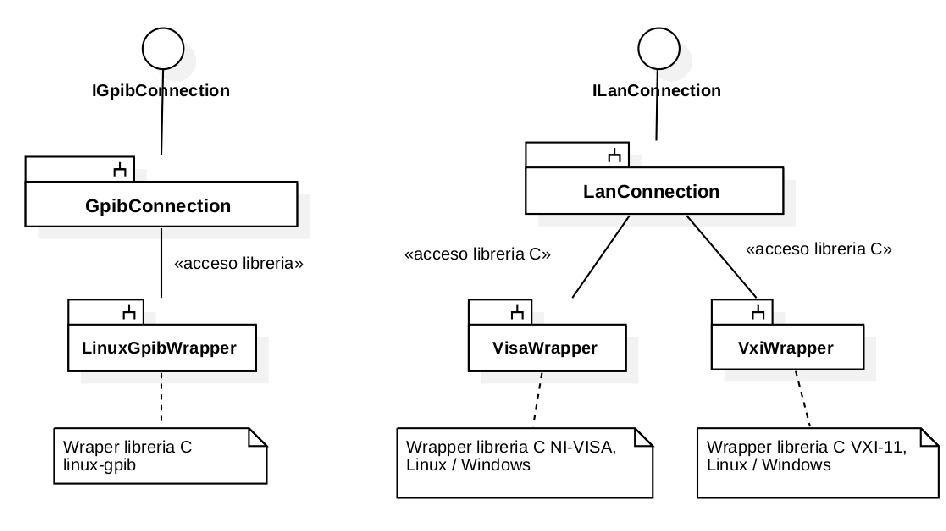
\includegraphics[width=0.8\textwidth]{Imagenes/CommunicationAbstractionLayerPackages2.pdf}
		\caption{Interfaces de software y sus dependencias, para conexión con buses Gpib y redes Lan}
		\label{Fig:CalPackages1}
	\end{figure}

	\begin{figure}[H]
		\centering
		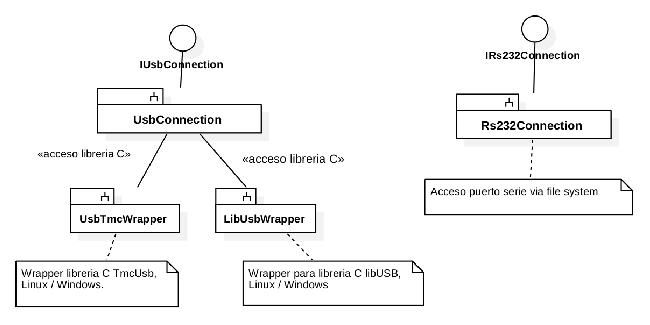
\includegraphics[width=0.8\textwidth]{Imagenes/CommunicationAbstractionLayerPackages3.pdf}
		\caption{Interfaces de software y sus dependencias, para conexión con buses Usb o Rs232}
		\label{Fig:CalPackages2}		
	\end{figure}
	
	\subsubsection{Interfaces de comunicaciones}
	
	Las interfaces de comunicaciones para la aplicación \AppName están representadas por el software de interfaz para los buses Gpib, Usb, Rs232 y el software de interfaz para acceso a redes Lan.
	
	
		% -----------------------------------------------------
		% Comando para generar formato con requisitos funcionales
		\newcommand{\funcreq}[7]{
			\subsubsection{Requerimiento funcional {#1}}

			\begin{table}[H]			
			%\begin{table}[!h]
				\begin{tabularx}{\textwidth}{rX}			
					\textbf{ID:} 	&	{#2}		\\
					Titulo:			&  	{#3}. 		\\
					Descripción:	&	{#4}.		\\
					Justificación: 	&	{#5}.		\\
					Dependencias:	& 	{#6}.		\\
					Usuario:		&	{#7}.		\\
				\end{tabularx}				
			\end{table}
		}
		% -----------------------------------------------------		
		
		% -----------------------------------------------------
		% Comando para generar formato con requisitos de desempeño
		\newcommand{\perfreq}[6]{
			\subsubsection{{Requerimiento de desempeño #1}}
			
			\begin{table}[H]
			%\begin{table}[!h]
				\begin{tabularx}{\textwidth}{rl}			
					\textbf{ID:} 	&	{#2}		\\
					Titulo:			&  	{#3}. 		\\
					Descripción:	&	{#4}.		\\
					Justificación: 	&	{#5}.		\\
					Dependencias:	& 	{#6}.		\\
				\end{tabularx}				
			\end{table}
		}
		% -----------------------------------------------------				
	
	\subsection{Requerimientos funcionales}	
	
	A continuación los requerimientos funcionales
	
	\funcreq{1}
		{FR1}
			{Instalar aplicación}
			{La aplicación requiere de una aplicación instalador}
			{Facilitar el proceso de instalación para el usuario}
			{Ninguna}
			{Técnico}
		
	\funcreq{1}
		{FR1}
			{Automatizar tareas de medición}
			{Los usuarios pueden programar los instrumentos y generar tareas de medición para sus posterior ejecución, de forma automatizada y remota}
			{Programar y automatizar las mediciones con el\SMR}
			{Ninguna}
			{Técnico}
	\funcreq{2} 
		{FR2}
			{Presentar una interfaz gráfica para el \SMR}
			{La aplicación servirá como una representación integral en software de los tres instrumentos principales que componen el \SMR, será un instrumento virtual}
			{Simplificar las tares de medición con el \SMR}
			{FR1}
			{Técnico}
	\funcreq{3}
		{FR3}
			{Gestión de las comunicaciones con los instrumentos del \SMR de manera simple y uniforme desde la perspectiva de usuario}
			{La aplicación facilitará el intercambio de datos con los instrumentos del \SMR}
			{Simplificar la adquisición de datos del \SMR}
			{FR1, FR2}
			{Técnico}				
	\funcreq{4}
		{FR4}
			{Gerencia de los instrumentos conectados a los buses}
			{La aplicación debe descubrir y enumerar los instrumentos conectados a los buses a los cuales el PC disponga de acceso}
			{Presentar al usuario los instrumentos disponibles en los buses}
			{Ninguna}
			{Técnico}
	\funcreq{5}			
		{FR5}
			{Presentar explorador y buscador de instrumentos al usuario}
			{Por medio de un control de GUI se presenta al usuario una lista visual de los instrumentos disponibles y en que bus se encuentran}
			{Presentar al usuario los instrumentos disponibles en los buses}
			{FR4}
			{Técnico}
	\funcreq{5}
		{FR5}
			{Configurar los instrumentos de medición}
			{Al usuario se le presentara una interfaz gráfica en donde podrá establecer la configuración de cada instrumento en linea}
			{Los instrumentos requieren una configuración previa antes de iniciar la medición}
			{FR2}
			{Técnico}
	\funcreq{6}
		{FR6}
			{Presentar al usuario las fases de cada tarea de medición}
			{Las tareas de medición se dividen en fases: busqueda de instrumentos, configuración de la tarea de medición, ejecución de la tarea de medición, configuración de presentación de resultados y presentación de resultados}
			{La aplicación guía al usuario desde el inicio hasta el final de la tarea de medición}
			{Ninguno}
			{Técnico}
	\funcreq{6}
		{FR6}
			{Mostrar una representación gráfica del montaje a utilizar para una tarea de medición, orientada a diagrama de bloques}
			{La aplicación permitirá al usuario describir de forma gráfica la interconexión de instrumentos para una tarea de medición}
			{Servir de ayuda gráfica al usuario para una tarea de medición}
			{FR2}
			{Técnico}
	\funcreq{7}
		{FR7}
			{Interfaz gráfica orientada a diagrama de bloques}
			{El usuario puede programar las tareas de medición por medio de la creación de diagramas de bloques, que representan funcionalidades diversas}
			{Con el objeto de automatizar el proceso de medición}	
			{Ninguna}		
			{Técnico}				
	\funcreq{8}
		{FR8}
			{Capacidad de programar el proceso medición}
			{El usuario puede elegir un conjunto de instrumentos y establecer una secuencia de comandos para estos, que podrá almacenar en disco y ejecutar en el futuro}
			{Con el objeto de automatizar los procesos de medición}
			{FR2, FR3, FR4 FR5}
			{Técnico}	
	\funcreq{9} 
		{FR9}
			{Capacidad para simular el proceso medición}
			{El usuario puede simular una tarea de instrumentación dada, sin necesidad de conexión con el \SMR}
			{Con el objeto de automatizar los procesos de medición}
			{FR2, FR3, FR4 FR5}
			{Técnico}			
	\funcreq{10}
		{FR11}
			{Capacidad para el montaje y configuración de tareas de medición}
			{El usuario puede salvar la configuración y programación que haya hecho sobre una tarea de medición}
			{Con el objeto de automatizar los procesos de medición}
			{FR3}
			{Técnico}								
	\funcreq{11}
		{FR11}
			{Capacidad para almacenar y cargar datos de calibración de instrumentos}
			{El usuario puede guardar almacenar los datos de calibración y cargarlos nuevamente antes de cada proceso de medición}
			{Con el objeto de automatizar los procesos de medición}
			{FR3}
			{Técnico}
	\funcreq{12}
		{FR12}
			{Capacidad de programar la secuencia de pasos en el proceso de medición}
			{El usuario podrá programar la secuencia de pasos a realizar en un proceso de medición dado}
			{Con el objecto de automatizar el proceso de medición}
			{FR2, FR3}	
			{Técnico}		
	\funcreq{13}
		{FR13}
			{Capacidad programar la presentación gráfica reporte con resultados de medición}
			{El usuario podrá escoger cuales de datos de las mediciones incluir en el reporte de salida. El usuario podrá configurar su presentación y disposición en el documento de salida}
			{Con el objeto de configurar el documento que presenta los resultados de medición}
			{FR3,FR4}
			{Técnico}		
			
	\subsection{Requerimientos de desempeño}	
	
	\perfreq{1}
		{QR1}
			{Diseño de interfaz gráfica limpio, descongestionado y ordenado}
			{La interfaz gráfica deberá presentar un diseño limpio y estructurado, con funcionalidad común agrupada en pantallas y el anidamiento de menús no sobrepasará de 2 niveles. Evitar la congestión de la interfaz gráfica.}
			{Con el objeto de facilitar la navegación por las pantallas de la aplicación}
			{Ninguna}
		
		\perfreq{2}
			{QR2}
				{La aplicación para PC deberá ser portable entre los SO Windows y Linux}
				{La aplicación debe ejecutarse de manera uniforme en los sistemas operativos Windows y Linux}
				{Facilitar al usuario el uso de la aplicación en ambos sistemas operativos.}
				{Ninguna}		
	
			
	\subsection{Restricciones de diseño}
	
	[Por completar]
	
	\subsection{Atributos del sistema de software}
	
	[Por completar]
	
	\section{Asignación de prioridades y plan de entregas}

	[Por completar]
	
	\subsection{Elección del método para asignar prioridades}
	
	[Por completar]
		
		
	\subsection{Plan de entregas}
	
	[Por completar]	
	
\end{document}